%% ----------------------------------------------------------------
%% Appendix: Machine-learning model hyper-parameters tuning
%% ----------------------------------------------------------------
%!TeX root = subfile
\label{chapter:appendixD}
\markboth{Appendix D Machine-learning model hyper-parameters tuning}{Appendix D Machine-learning model hyper-parameters tuning}
\documentclass[../main.tex]{subfiles}
% ---------------------------------------------------------------- 
\begin{document}
A hyper-parametric study of the proposed ML model for the SANS equations is performed next.
Different MIMO-CNN architectures are considered, as shown in \fref{fig:cnn}.
All of the different CNNs are based on encoding the input information into some lower-dimensional latent space followed by a decoding procedure that maps such latent space into the target outputs, similarly to SegNet \citep{Badrinarayanan2015} or U-net \citep{Ronneberger2015} architectures.

For the hyper-parametric study, a dataset of 10152 snapshots containing the resolved quantities $\left\lbrace U, V, P \right\rbrace$ and the residual closure terms $\lbrace \mathcal{S}^R_x,\mathcal{S}^R_y\rbrace$ is generated throughout approximately 600 wake cycles.
The size of the recorded 2-D flow fields is $1216\times540$.
The data is split 80-20 for training and testing, respectively.
The training data is further split 75-25 for optimisation and validation, respectively.
The test dataset is generated after the 600 wake cycles, hence this data is completely hidden from the CNN during the training stage.
Only the inner uniform domain (see \fref{fig:computational_domain}) is stored during the data generation process.
For the training stage, an early-stopping approach is considered as the convergence criteria when the validation loss does not improve for 8 consecutive epochs (dataset iterations), or a maximum of 200 epochs is reached.
Success is measured by the Pearson correlation coefficient between the target $({\mathcal{S}}^{R})$ and predicted $(\mathcal{S}^{R,\,\mathrm{ML}})$ output fields, respectively
\begin{gather}
\mathcal{CC}_x=\mathcal{CC}\pars{\mathcal{S}^R_x,\mathcal{S}_x^{R,\,\mathrm{ML}}}=\frac{\mathrm{cov}\pars{\mathcal{S}^R_x,\mathcal{S}_x^{R,\,\mathrm{ML}}}}{\sqrt{\mathrm{cov}\pars{\mathcal{S}^R_x,\mathcal{S}^R_x}\mathrm{cov}\pars{\mathcal{S}_x^{R,\,\mathrm{ML}},\mathcal{S}_x^{R,\,\mathrm{ML}}}}},\\
\mathcal{CC}_y=\mathcal{CC}\pars{\mathcal{S}^R_y,\mathcal{S}_y^{R,\,\mathrm{ML}}}=\frac{\mathrm{cov}\pars{\mathcal{S}^R_y,\mathcal{S}_y^{R,\,\mathrm{ML}}}}{\sqrt{\mathrm{cov}\pars{\mathcal{S}^R_y,\mathcal{S}^R_y}\mathrm{cov}\pars{\mathcal{S}_y^{R,\,\mathrm{ML}},\mathcal{S}_y^{R,\,\mathrm{ML}}}}}.
\end{gather}

A mini-batch gradient descend method (4 to 6 samples depending on the GPU memory) using the Adam optimiser \citep{Kingma2014} is employed.
The learning rate is set to $10^{-4}$ with a decay rate of $10^{-5}$.
The full model is developed under Keras \citep{Chollet2015}, a deep-learning Python library using the TensorFlow \citep{Tensorflow} backend.

Because of the network weights are initialised randomly and stochastic gradient descent backpropagation is used to optimise the network, there is an irreducible level of randomness in the final results.
Hence, the training process is repeated for cases converged into a very shallow local minima and only the best results have been reported.

A flow field snapshot of resolved quantities and a target output is displayed in \fref{fig:flow_field}.
The complex flow structures at the shear layer roll-up region behind the cylinder can be particularly challenging to model.
This can indicate that a large CNN in terms of number of trainable parameters (weights $\matr{W}$ and bias $\vect{b}$) is required.
Also, beyond exploring different CNN architectures, we test different loss functions, activation functions, number of filters and kernel size, effect of input data normalisation, and different input sets.
A summary of the parametric study is detailed in \tref{tab:parameters} and the base-case parameters are shown in \tref{tab:models_fixed_parameters}.

\begin{table}
\begin{center}
\begin{tabular}{ll}
\toprule
Architecture & M1, M2, M3\\
Loss function & sse, sae \\
Activation function & ReLU, tanh, sigmoid \\
Max. filters & 16, 32, 64 \\
Kernel size & $3\times3, \,\,\, 5\times5, \,\,\,7\times7$ \\
Normalised input data & False, True \\
Input set & $\left\lbrace U, V, P \right\rbrace$, $\left\lbrace \Omega_z, d \right\rbrace$,  $\left\lbrace \nabla\vect{U}, \nabla P \right\rbrace$ \\
\bottomrule
\end{tabular}
\end{center}
\caption{Parametric study.
sse: sum square error.
sae: sum absolute error.
ReLU: rectified linear unit.
$\Omega_z$: Spanwise-averaged vorticity.
$d$: Distance function to the cylinder.}
\label{tab:parameters}
\end{table} 

\begin{table}
\begin{center}
\begin{tabular}{ll}
\toprule
Architecture & M3 \\
Loss function & sse \\
Activation function & ReLU \\
Max. filters & 64 \\
Kernel size & $3\times3$ \\
Normalised input data & True \\
Input set & $\left\lbrace U, V, P \right\rbrace$ \\
\bottomrule
\end{tabular}
\end{center}
\caption{Base-case parameters of the parametric investigation.}
\label{tab:models_fixed_parameters}
\end{table}

\clearpage
\begin{figure}[!h]
	\centering
	\begin{subfigure}[t]{\linewidth}		
		\centering
		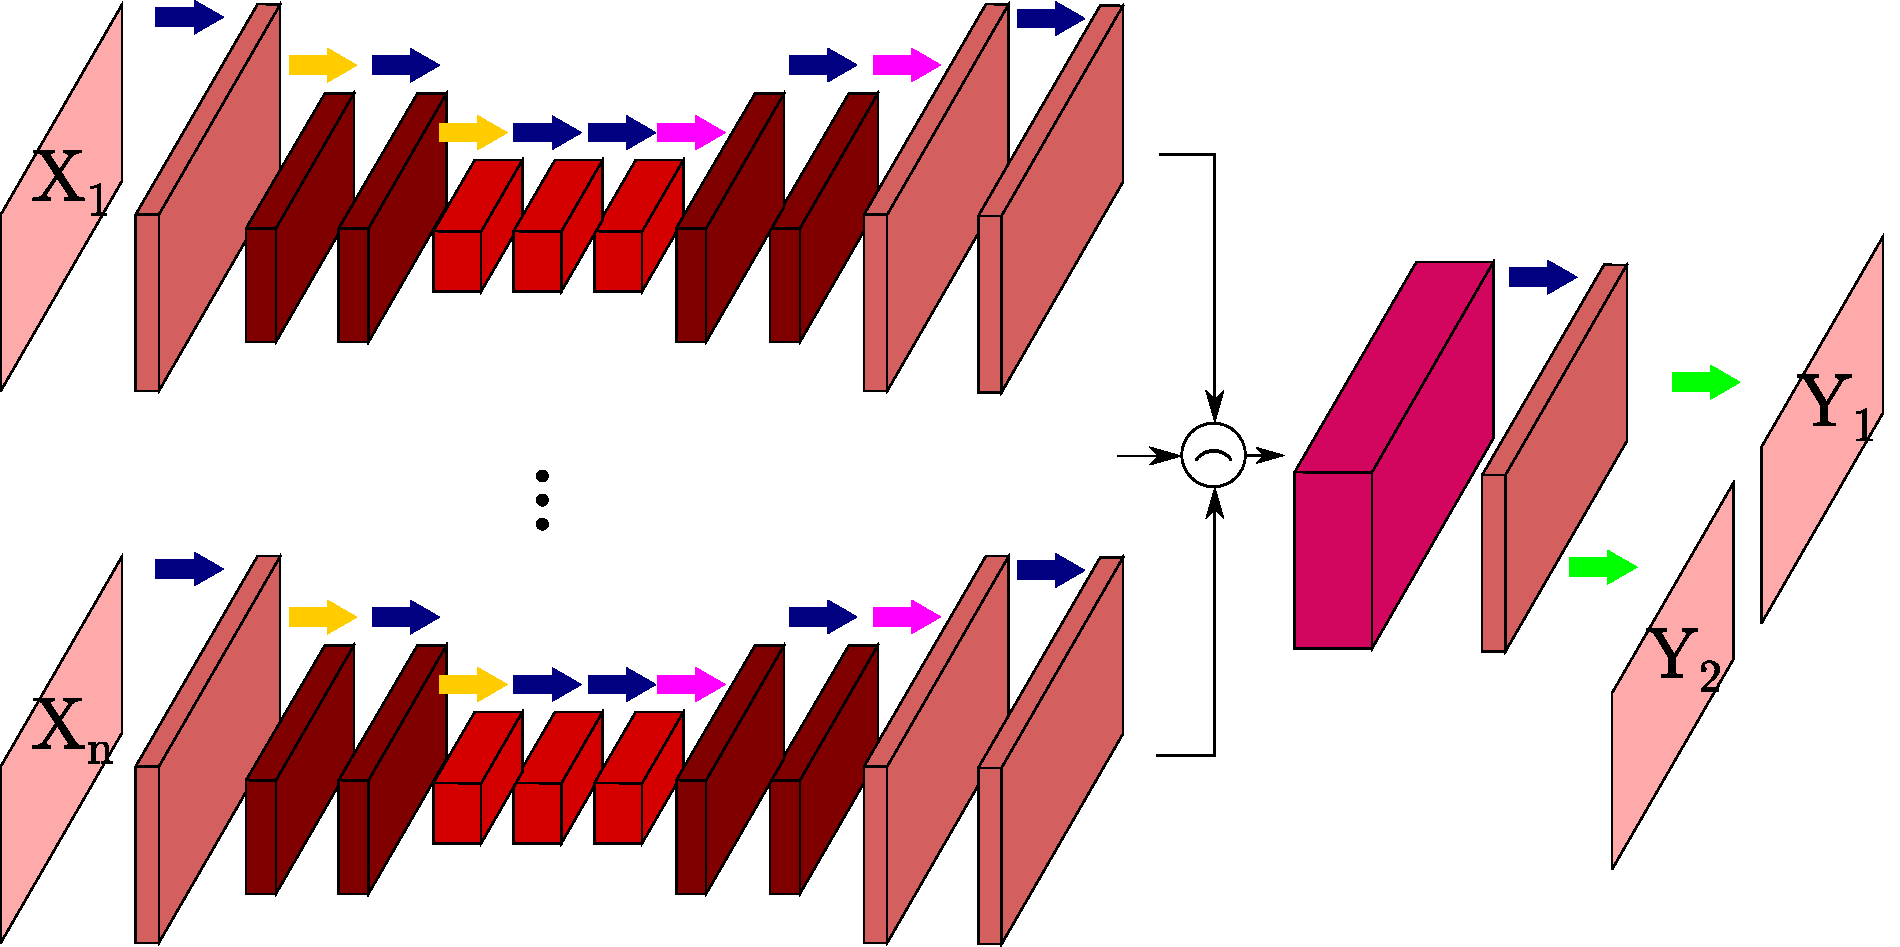
\includegraphics[width=0.7\linewidth]{appendixD/cnn/cnn_1.pdf}%
		\caption{Model 1 (M1)}\vspace{0.7cm}
	\end{subfigure}
	\begin{subfigure}[t]{\linewidth}
		\centering
		\vspace{0.5cm}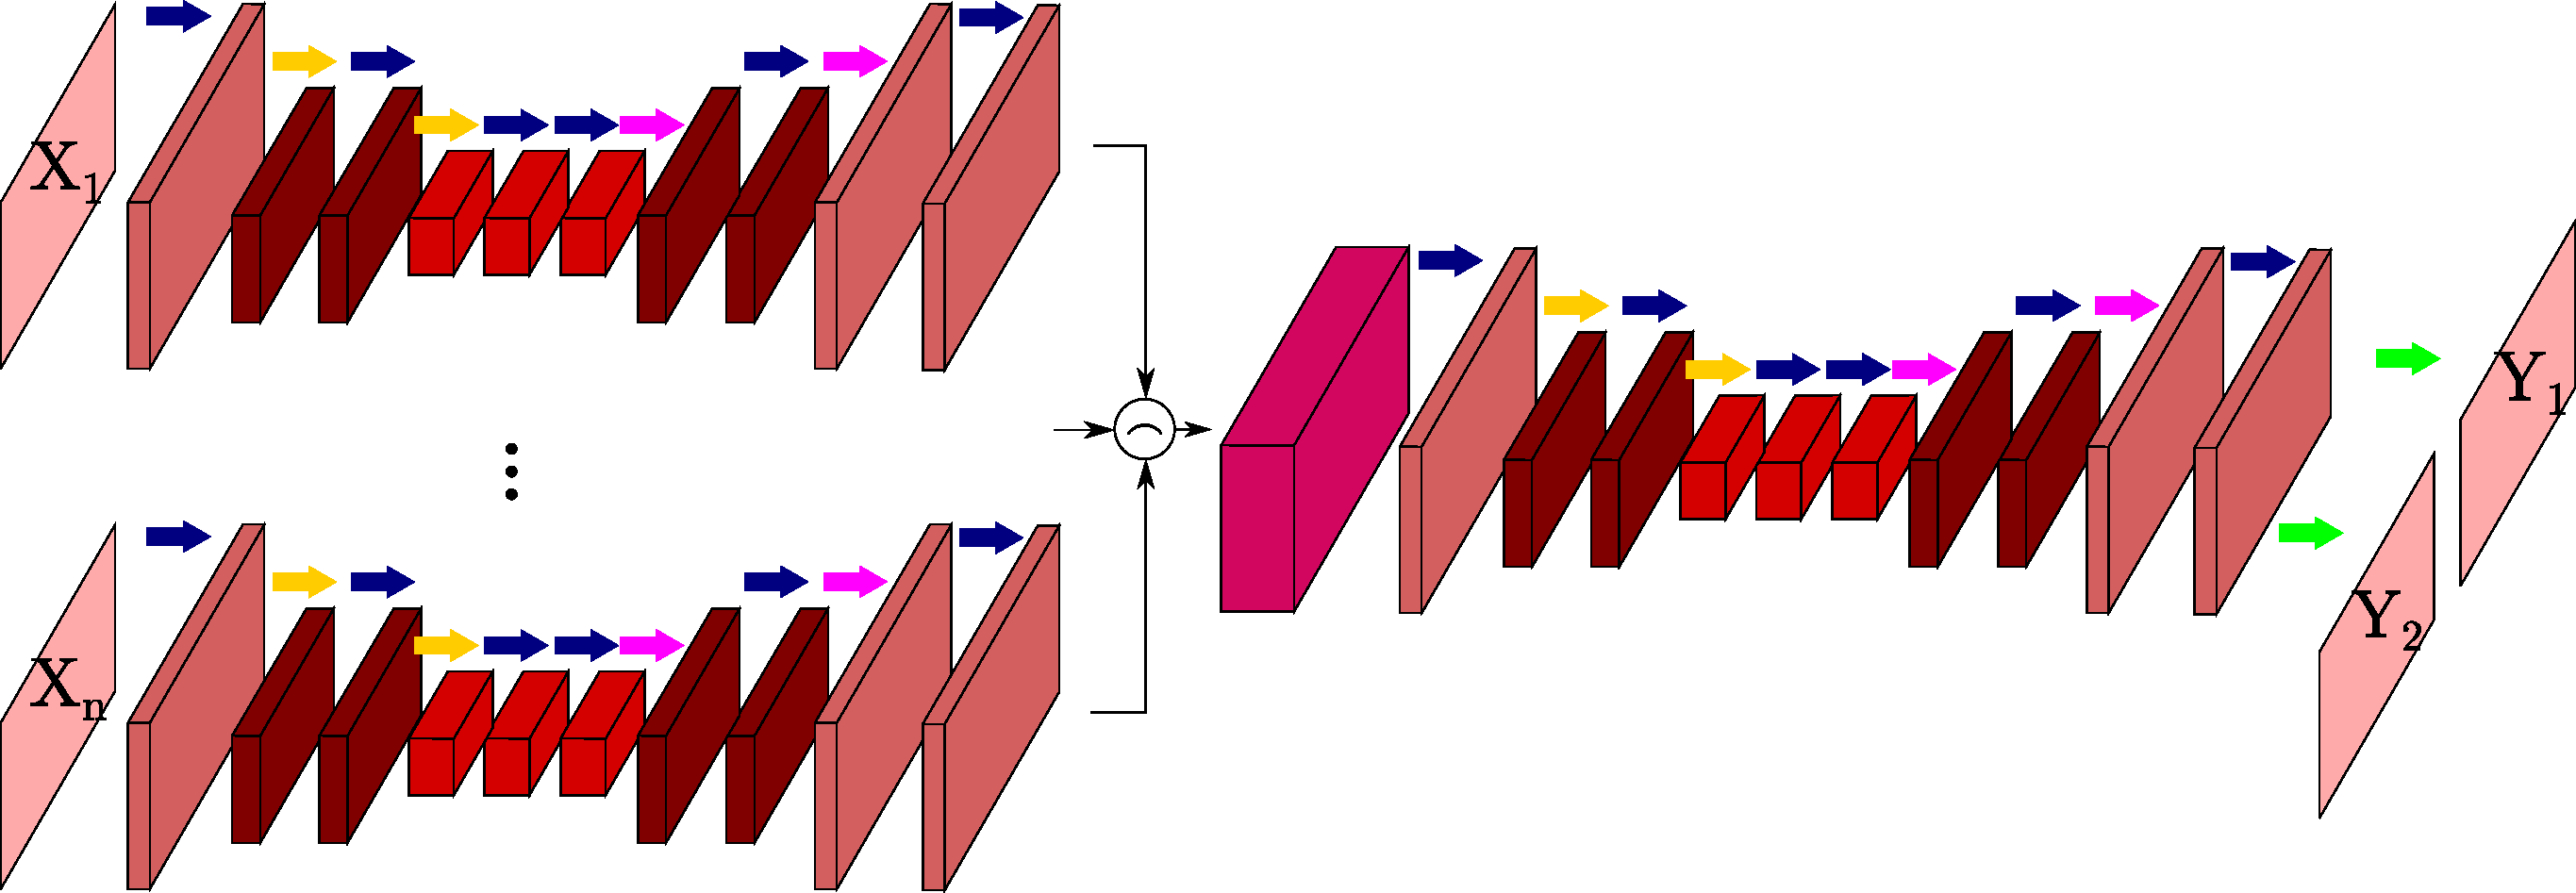
\includegraphics[width=0.95\linewidth]{appendixD/cnn/cnn_2.pdf}%
		\caption{Model 2 (M2)}\vspace{0.9cm}
	\end{subfigure}
	\begin{subfigure}[t]{\linewidth}
		\centering
		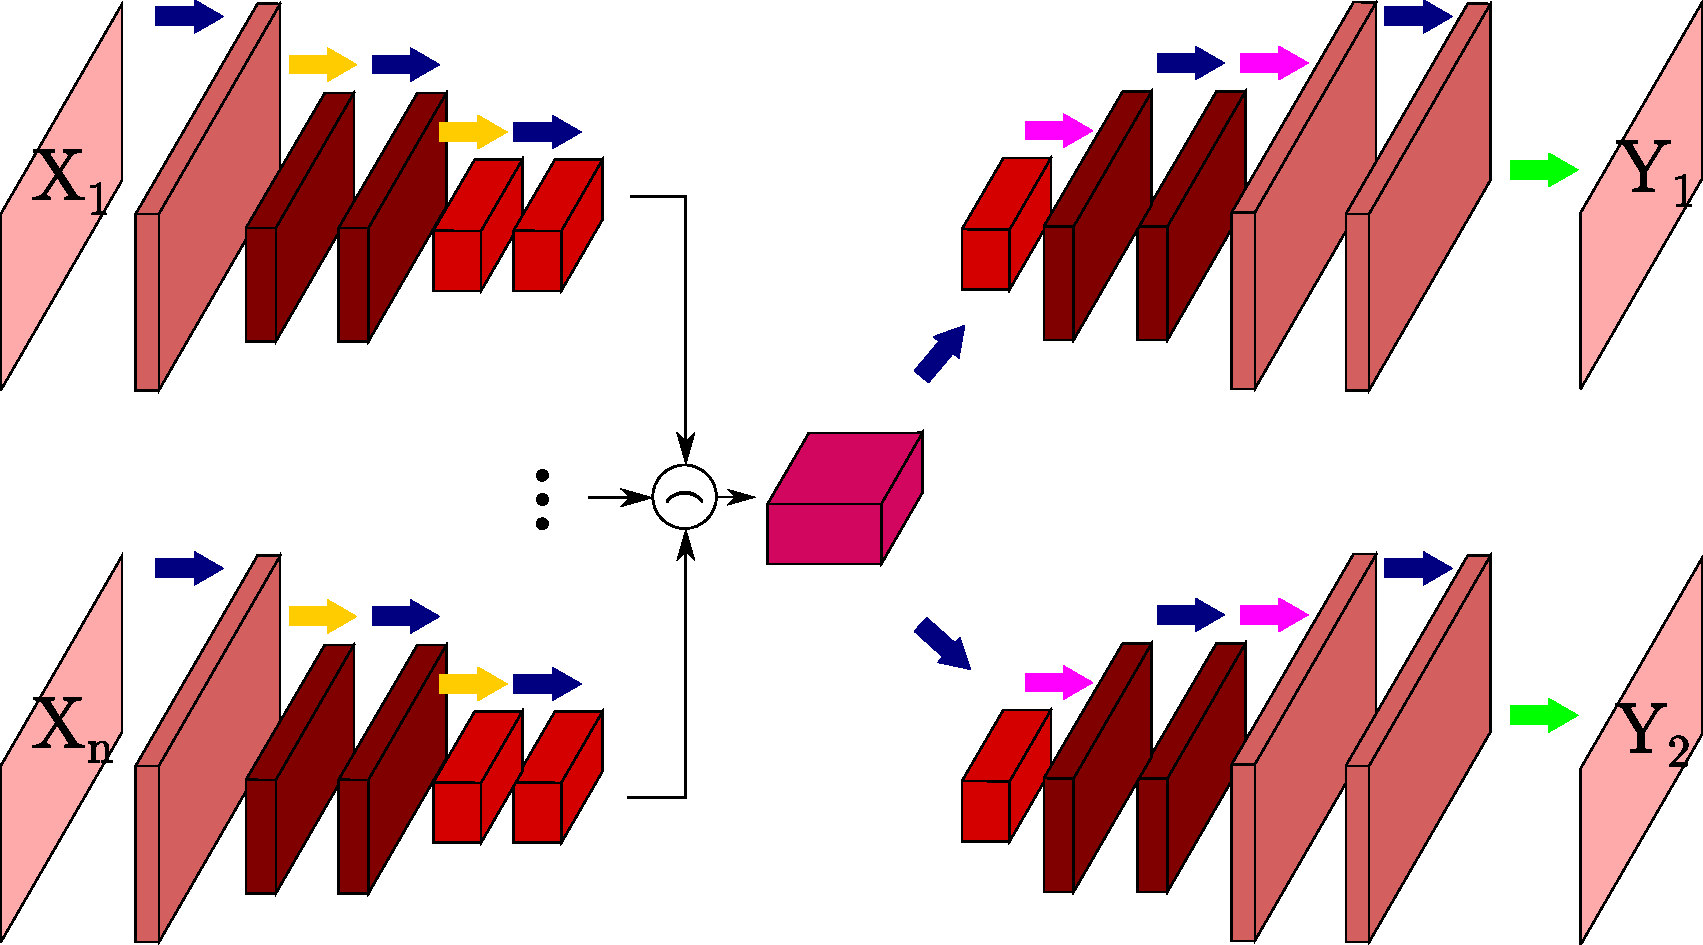
\includegraphics[width=0.6\linewidth]{appendixD/cnn/cnn_3.pdf}%
		\caption{Model 3 (M3)}
	\end{subfigure}
	\captionsetup[subfigure]{width=\linewidth}
	\caption{CNN architectures investigated.
The input $(\mathrm{X}_n)$ and output $(\mathrm{Y}_n)$ fields size is $1216\times540$.
Arrows color indicate layers of:
Dark blue: Conv2D $+$ batch normalisation $+$ activation function.
Yellow: MaxPooling $2\times2$.
Magenta: UpSampling $2\times2$.
Green: Conv2D $1\times1$ $+$ batch normalisation $+$ linear function.
The thickness of each block (noted on the last dimension) represents the number of filters.
On the encoding blocks, the number of filters is doubled at every convolutional layer, reaching a maximum number of filters just before the decoding block, where the operation is reversed halving the number of filters at every convolutional layer.
The merging operator $\frown$ indicates concatenation in the last dimension, hence stacking filters from multiple blocks.}\label{fig:cnn}
\end{figure}


\begin{figure}
	\centering
	\captionsetup[subfigure]{width=1\linewidth}
	\begin{subfigure}[t]{0.9\linewidth}		
		\centering
		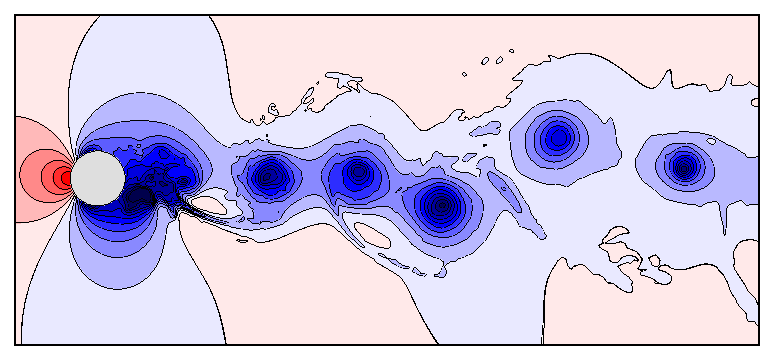
\includegraphics[width=\linewidth]{appendixD/flow_field/P.pdf}%
	\caption{$P$}
	\end{subfigure}
	\begin{subfigure}[t]{\linewidth}		
		\centering
		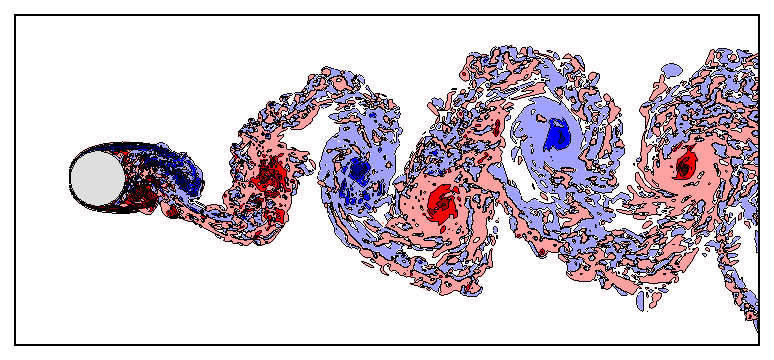
\includegraphics[width=0.9\linewidth]{appendixD/flow_field/vort_lowres.pdf}%
	\caption{$\Omega_z$}
	\end{subfigure}
	\begin{subfigure}[t]{\linewidth}
		\centering
		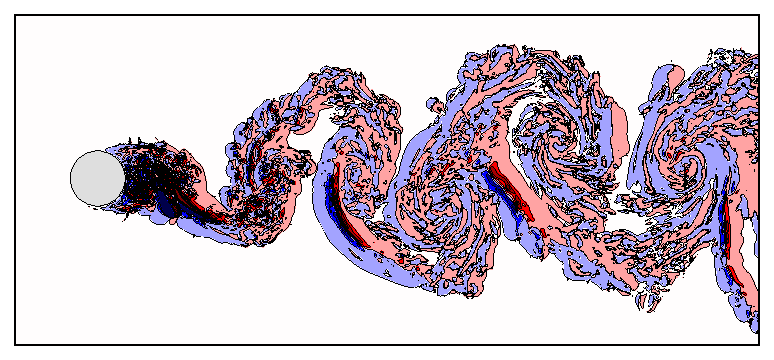
\includegraphics[width=0.9\linewidth]{appendixD/flow_field/tau_x_lowres.pdf}%
		\caption{$\mathcal{S}^R_x$}
	\end{subfigure}
	\caption{Flow snapshot of resolved (top, middle) and target closure (bottom) fields.} \label{fig:flow_field}
\end{figure}

\section{Results}

\subsection{Model architecture and data normalisation}

We start investigating the CNN architecture based on three different models, namely M1, M2 and M3 (see \fref{fig:cnn}).
The base-case parameters are detailed in \tref{tab:models_fixed_parameters}.
We also study the effect of normalising each input data sample with its standard score, i.e. $\hat{x} = \pars{x-\bar{x}}/\sigma_x$.

Results for the training stage of each model are displayed in \fref{fig:models_convergence}.
It can be observed that normalising the input data provides a faster convergence, noting that the non-normalised M1 case hits the maximum number of epochs limit.
The correlation coefficient results are given in \tref{tab:models_correlation}.
All models provide a high correlation coefficient for both validation and test datasets (hence no over-fitting is detected).
The general trend is that accuracy increases with the network size.
It is expected that output decoding branches having access to a larger latent space (number of filters encoding information on the encoder output), such as M3, are more flexible and perform better than networks with a smaller latent space.
The M3 model with normalised input data is selected for all the subsequent analysis, unless specified otherwise.
The choice is motivated by the M3 model training consistency and its slightly faster convergence when compared to other models.

{\renewcommand{\arraystretch}{1.2}
\begin{table}[t]
\begin{center}
\begin{tabular}{ccccc}
\toprule
Case & \specialcell{Train.\\params.} & val.: $\mathcal{CC}_x,\,\mathcal{CC}_y$ & test: $\mathcal{CC}_x,\,\mathcal{CC}_y$ & Best epoch\\
\midrule
M1 & 258242 & 0.75, 0.83 &  0.74, 0.83 & 200\\
\specialcell{M1\\norm.} & 258242 & 0.84, 0.85 & 0.83, 0.84 & 70\\
M2 & 300194 & 0.85, 0.86 & 0.84, 0.84 & 81\\
\specialcell{M2\\norm.} & 300194 & {0.86, 0.88} & {0.85, 0.88}& 62\\
\specialcell{M2\\norm.\\stacked} & 58538 & 0.76, 0.77 &  0.74, 0.76 & 63\\
M3 & 338498 & 0.87, 0.88 & 0.86, 0.87 & 105\\
\specialcell{M3\\norm.} & 338498 & 0.86, 0.85 & 0.85, 0.84 & 70\\
\bottomrule
\end{tabular}
\end{center}
\caption{Validation and test results for different model architectures.}
\label{tab:models_correlation}
\end{table}}

\clearpage
\begin{figure*}[!ht]
\centering
\vspace{1cm}
\begin{multicols}{2}
	\begin{subfigure}[t]{\linewidth}		
		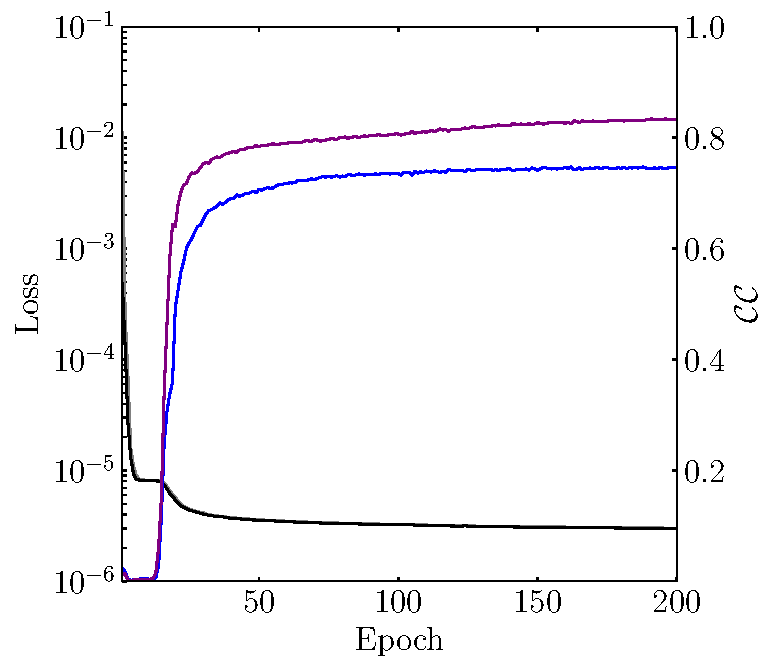
\includegraphics[width=\linewidth]{appendixD/history/1.pdf}%
		\caption{M1}
	\end{subfigure}\vspace{0.3cm}
	\begin{subfigure}[t]{\linewidth}		
		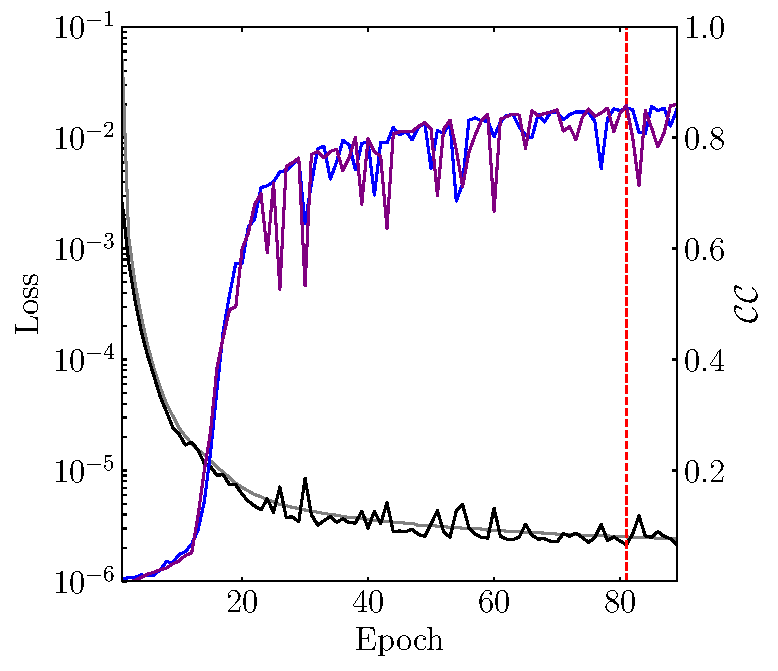
\includegraphics[width=\linewidth]{appendixD/history/3.pdf}%
		\caption{M2}
	\end{subfigure}\vspace{0.3cm}
	\begin{subfigure}[t]{\linewidth}
		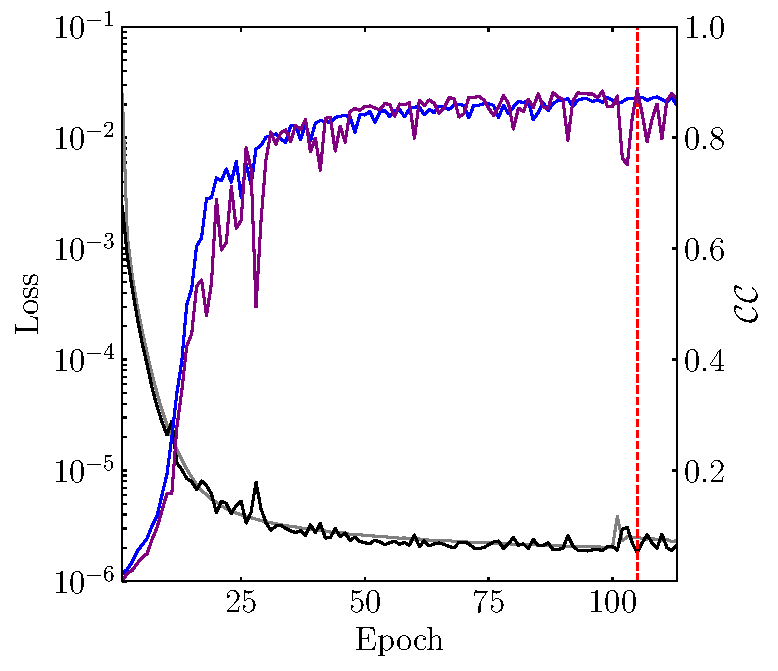
\includegraphics[width=\linewidth]{appendixD/history/5.pdf}
		\caption{M3}
	\end{subfigure}
		\begin{subfigure}[t]{\linewidth}		
		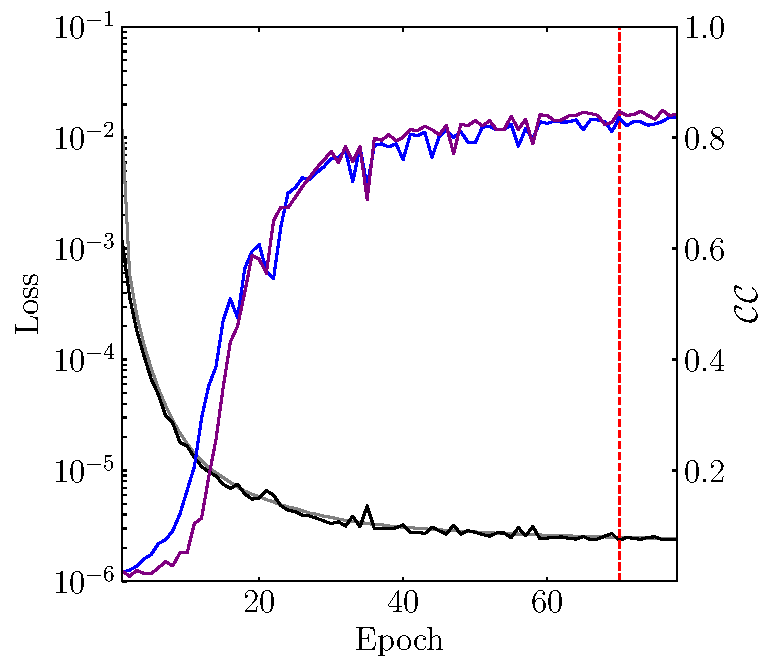
\includegraphics[width=\linewidth]{appendixD/history/2.pdf}%
		\caption{M1, norm.}
	\end{subfigure}\vspace{0.3cm}
		\begin{subfigure}[t]{\linewidth}		
		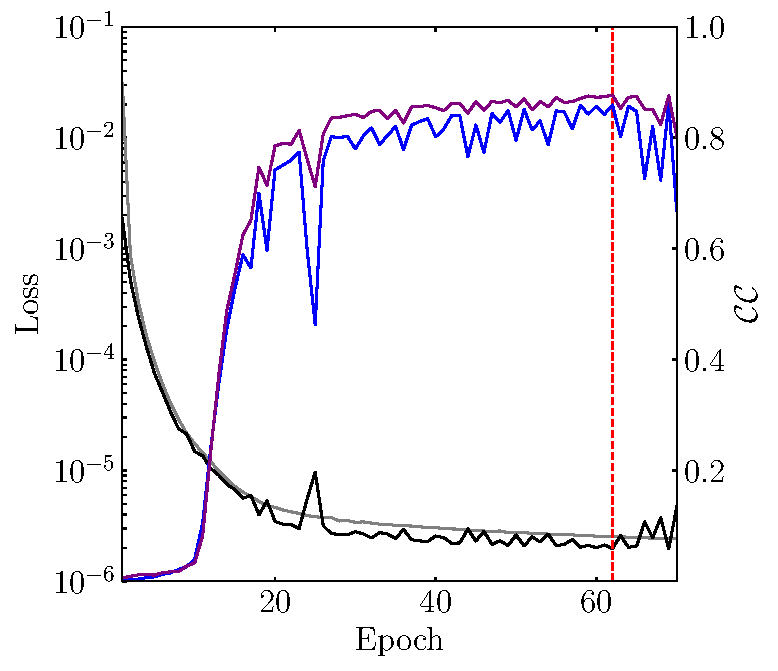
\includegraphics[width=\linewidth]{appendixD/history/4.pdf}%
		\caption{M2, norm}
	\end{subfigure}\vspace{0.3cm}
	\begin{subfigure}[t]{\linewidth}		
		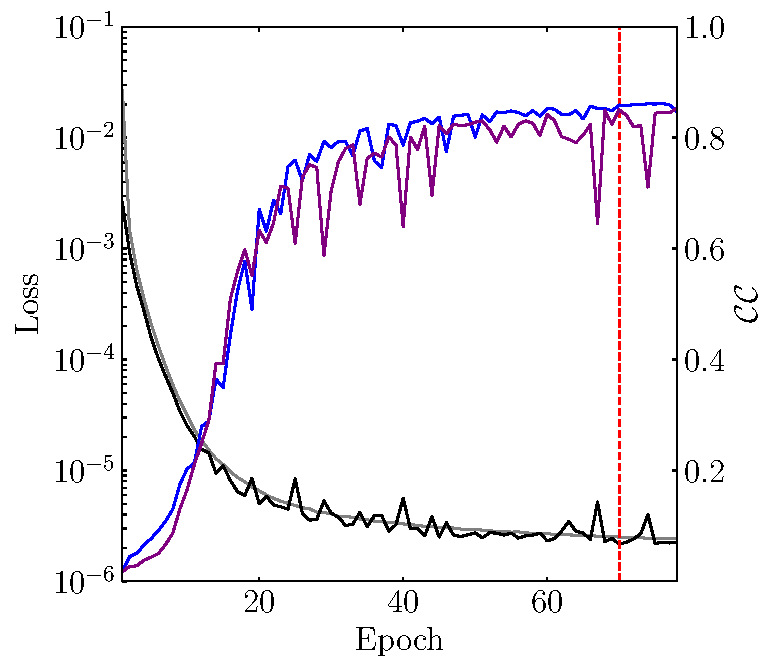
\includegraphics[width=\linewidth]{appendixD/history/6.pdf}%
		\caption{M3, norm.}
	\end{subfigure}
\end{multicols}
	\caption{Training history of the different model architectures.
Left: Input data not normalised.
Right: Input data normalised.
Legend: Grey: fit loss.
Black: val. loss.
Blue: $\mathcal{CC}_x$ (val. dataset).
Purple: $\mathcal{CC}_y$ (val. dataset).
Red: Early stop mark.} 
	\label{fig:models_convergence}
\end{figure*}

\clearpage
Additionally, a simple auto-encoder concatenating the resolved quantities in a single input branch (stacking them in the filter dimension, noted in \tref{tab:models_correlation} as ``stacked'') has been tested.
Even though this model is much smaller than the other ones in terms of number of trainable parameters, it still manages to provide acceptable predictions.

\subsection{Loss function}

The loss function between predicted and target fields is investigated next.
The same previous base-case parameters are chosen and results are summarised in \tref{tab:loss_correlation}.

{\renewcommand{\arraystretch}{1.2}
\begin{table}
\begin{center}
\begin{tabular}{ccccc}
\toprule
Case & \specialcell{Train.\\params.} & val.: $\mathcal{CC}_x,\,\mathcal{CC}_y$ & test: $\mathcal{CC}_x,\,\mathcal{CC}_y$ & Best epoch\\
\midrule
sse & 338498 & 0.86, 0.85 & 0.85, 0.84 & 70 \\
sae & 338498 & 0.86, 0.57 & 0.83, 0.48 & 45\\
\bottomrule
\end{tabular}
\end{center}
\caption{Validation and test results for different loss functions.}
\label{tab:loss_correlation}
\end{table}}

It can be observed that using the absolute error yields to a local minima where one of the outputs has not converged successfully.
The squared error function being an easier metric to differentiate (convex parabola) than the absolute error might be causing such difference.

\subsection{Activation function}

Activation functions ($h$) are used to dictate the output of a neuron based on some input value $x$ (the model input or a previous layer output), a weight and a bias: $a = h(wx+b)$.
Activation functions widely used in ANNs are tested here.
We consider the ReLU, tanh, and sigmoid activation functions.
Results are displayed in \tref{tab:activation_correlation}.

It can be observed that the ReLU activation function provides a clear advantage in comparison with the other tested functions.
The ReLU function allows for faster trainings of deep ANNs because it preserves the neuron relative intensity across layers (maximum value is not capped) \citep{Nair2010}.
This is also due to the fact that the ReLU function helps mitigating vanishing-gradient caveats which arise more naturally when using the sigmoid function.

{\renewcommand{\arraystretch}{1.2}
\begin{table}
\begin{center}
\begin{tabular}{ccccc}
\toprule
Case & \specialcell{Train.\\params.} & val.: $\mathcal{CC}_x,\,\mathcal{CC}_y$ & test: $\mathcal{CC}_x,\,\mathcal{CC}_y$ & Best epoch\\
\midrule
ReLU & 338498 & 0.86, 0.85 & 0.85, 0.84 & 70 \\
tanh & 338498 & 0.78, 0.76 & 0.77, 0.76 & 62\\
sigmoid & 338498 & 0.81, 0.82 & 0.80, 0.82 & 36\\
\bottomrule
\end{tabular}
\end{center}
\caption{Validation and test results for different activation functions.}
\label{tab:activation_correlation}
\end{table}}

\subsection{Number of filters and kernel size}

The number of filters per convolutional layer and the convolution kernel size is explored.
The results for the maximum number of filters per convolutional layer are displayed in \tref{tab:filters_correlation}, where the number of trainable parameters jumps by a factor of 4.
The results observed in this particular study are strongly biased by the number of training epochs.
It should be noted that the case using a maximum of 16 filters only converged after almost 400 epochs (the maximum epochs limit has been lifted here because of the network size), whereas the other cases are both converged under 100 epochs.
The slow convergence of the 16 filters might be due to its lack of flexibility (model degrees of freedom) compared to the models with more filters available.
Still, the 64 filters case displays correlation coefficients relatively close to the 16 filters case with only 70 epochs of training.
Hence it can be argued that increasing the number of filters allows the model to be optimised based on a wider range of spatial features thus achieving a faster convergence.
Simultaneously, increasing the number of filters does not automatically yield better accuracy.

From a computational cost standpoint, the training time for the 64 maximum filters case is approximately 26 min./epoch, whereas the 32 and 16 filters cases are both around 23 min./epoch (the latter only measured during its first 100 epochs).
Hence, the computational cost does not increase linearly with the network size.
On the other hand, the computational training time of the 16 filters case gradually increases with every new epoch.
For the 378 epochs until convergence, a total of 180 hours of computational time is required, averaging to roughly 28 min./epoch.
Therefore, the computational time per epoch increases with the number of epochs, making the 16 maximum filters case less efficient compared to the larger networks.

{\renewcommand{\arraystretch}{1.2}
\begin{table}
\begin{center}
\begin{tabular}{ccccc}
\toprule
Case & \specialcell{Train.\\params.} & val.: $\mathcal{CC}_x,\,\mathcal{CC}_y$ & test: $\mathcal{CC}_x,\,\mathcal{CC}_y$ & Best epoch\\
\midrule
64 & 338498 & 0.86, 0.85 & 0.85, 0.84  & 70\\
32 & 85154 & 0.81, 0.72 & 0.81, 0.71 & 34\\
16 & 21554 & 0.87, 0.87 & 0.87, 0.86 & 386\\
\bottomrule
\end{tabular}
\end{center}
\caption{Validation and test results for different maximum number of filters.}
\label{tab:filters_correlation}
\end{table}}

{\renewcommand{\arraystretch}{1.2}
\begin{table}
\begin{center}
\begin{tabular}{ccccc}
\toprule
Case & \specialcell{Train.\\params.} & val.: $\mathcal{CC}_x,\,\mathcal{CC}_y$ & test: $\mathcal{CC}_x,\,\mathcal{CC}_y$ & Best epoch\\
\midrule
$3\times3$ & 338498 & 0.85, 0.86 & 0.86, 0.84 & 70 \\
$5\times5$ & 937282 & 0.89, 0.89 & 0.89, 0.89 & 101\\
$7\times7$ & 1835458 & 0.87, 0.86 & 0.86, 0.86 & 34\\
\bottomrule
\end{tabular}
\end{center}
\caption{Validation and test results for different kernel sizes.}
\label{tab:kernels_correlation}
\end{table}}

The results for the kernel size effect are displayed in \tref{tab:kernels_correlation}.
The kernel size is important for the detection of small- and large-scale structures.
The kernel size to capture the smallest scale in the wake should be, at least, a $3\times3$ filter since our iLES solver is resolving spatial scales down to grid level.
Structures larger than the grid-level scale might be better identified by slightly larger kernels.
However, the nonlinear combination of feature maps across the CNN layers allows small kernels to reconstruct such large-scale structures, hence the implied advantage of slightly larger kernels is not as relevant.
On the other hand, large kernels will filter out information of the subkernel-scale structures.
This is why the current accepted practice in CNNs is to use either $3\times3$ or $5\times5$ kernels and our results agree with that practice.
The $5\times5$ kernel configuration provides the best prediction among the kernels set, where a compromise between the detection of small- and large-scale structures is achieved.

\subsection{Input data}

Last, different input sets are evaluated.
Here, we consider the M2 model without normalising the inputs.
This is motivated by the fact that the M3 model becomes very large when 6 different inputs are used, as it is the case with the $\left\lbrace \nabla\vect{U}, \nabla P \right\rbrace$ input set.
The remaining base-case parameters are employed.
By testing different inputs we seek to include features more closely related to the expected outputs so that the regression problem solved by the CNN becomes easier \citep{Gamahara2017, Beck2019}.

As summarised in \tref{tab:inputs_correlation}, it is found that the primitive quantities set and the gradient set provide the highest correlation between target and predicted closure terms.
On the other hand, the vorticity plus the distance function input set does not perform as well.
The closure terms are, in their core, convective terms of the spanwise-fluctuating velocity field.
Hence, it is reasonable to argue that spatial derivatives of the resolved spanwise-averaged velocity field carry more relevant information to the closure terms than the other input sets.
Still, the primitive quantities set performs very similarly to the gradient set.
This can be an indicator of the network being able to find the gradients on its own.
Also, compared to the vorticity input set, it seems that information on the pressure field is important although this has not been tested in direct comparison.

{\renewcommand{\arraystretch}{1.2}
\begin{table}
\begin{center}
\begin{tabular}{ccccc}
\toprule
Case & \specialcell{Train.\\params.} & val.: $\mathcal{CC}_x,\,\mathcal{CC}_y$ & test: $\mathcal{CC}_x,\,\mathcal{CC}_y$ & Best epoch\\
\midrule
$\left\lbrace U, V, P \right\rbrace$& 338498 & 0.86, 0.85 & 0.85, 0.84 & 70\\
$\left\lbrace \Omega_z, d \right\rbrace$& 255746 & 0.57, 0.52  & 0.56, 0.52 & 110\\
$\left\lbrace \nabla\vect{U}, \nabla P \right\rbrace$ & 433538 & 0.86, 0.87 & 0.85, 0.86 & 112\\
\bottomrule
\end{tabular}
\end{center}
\caption{Validation and test results for different input sets.}
\label{tab:inputs_correlation}
\end{table}}

\section{Conclusion}

The M2 model has provided the highest correlations across the tested models for a given set of base-case parameters, and, on the other hand, the M3 model offered the best consistency while training.
Also, normalising the input data allows for faster training convergence without significantly compromising accuracy.
The sse loss function, a maximum of 64 filters, and a kernel size of $5\times5$ proved to be the best possible parameters.
Finally, the gradient input set and the primitive quantities set performed similarly providing the highest correlation coefficients (see \tref{tab:best_model}).

From a qualitative standpoint, predictions and target closure terms are displayed in \fref{fig:predictions}.
The M3 model using the normalised primitive quantities input set, a kernel size of $5\times5$, the sse loss function, and 64 maximum filters has been employed to generate the predicted closure terms (highest $\mathcal{CC}$ observed: $\mathcal{CC}(\mathcal{S}^R_x)=0.89,\, \mathcal{CC}(\mathcal{S}^R_y)=0.89$).
The predicted fields have been post-processed including a wake mask step constructed from the resolved vorticity field and a Gaussian filter to mitigate the noise in the raw CNN output (note that all the presented correlation values do not include this post-processing step).
This post-processing step is similar to process described in \sref{sec:ML_model} although in that case it is embedded in the CNN.

\fref{fig:predictions} shows that both large- and mid-scale structures are well captured by the model.
On the other hand, small-scale structures are not so well identified.
Similar issues are encountered in \cite{Lee2019}, where deep-learning models employed for recursively generating snapshots of flow past a circular cylinder at high $Re$ failed to fully reproduce small-scale structures.
Also, the noise observed in the $\mathcal{S}^{R,\,\mathrm{ML}}_y$ output motivates the inclusion of a wake mask, as described in \sref{sec:ML_model}.

{\renewcommand{\arraystretch}{1.2}
\begin{table}
\begin{center}
\begin{tabular}{ll}
\toprule
Architecture &\noindent \specialcell{M2 (highest correlation)\\M3 (best training consistency)} \\
Loss function & sse \\
Activation function & ReLU \\
Max. filters & 64 \\
Kernel size & $5\times5$ \\
Normalise input data & True \\
Input dataset & $\left\lbrace U, V, P \right\rbrace$, $\left\lbrace \nabla\vect{U}, \nabla P \right\rbrace$\\
\bottomrule
\end{tabular}
\end{center}
\caption{Summary of best results.}
\label{tab:best_model}
\end{table}}

\begin{figure*}[!ht]
\begin{multicols}{2}
\begin{subfigure}[t]{\linewidth}
    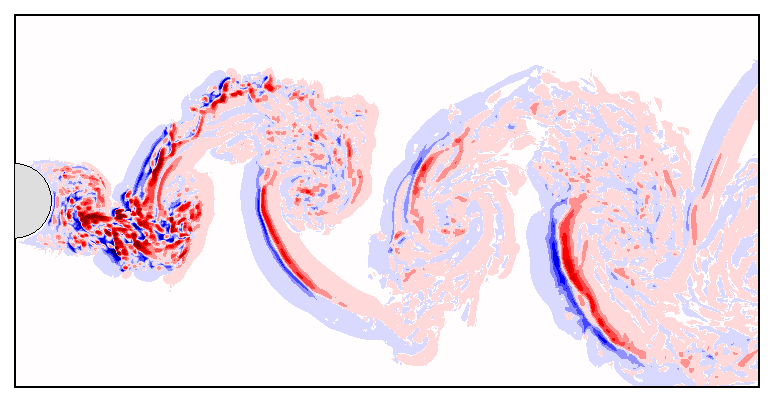
\includegraphics[width=\linewidth]{appendixD/predictions/SR_x_3693.0.pdf}\caption{$\mathcal{S}^R_x$} 
\end{subfigure}\vspace{0.5cm}
\begin{subfigure}[t]{\linewidth}
    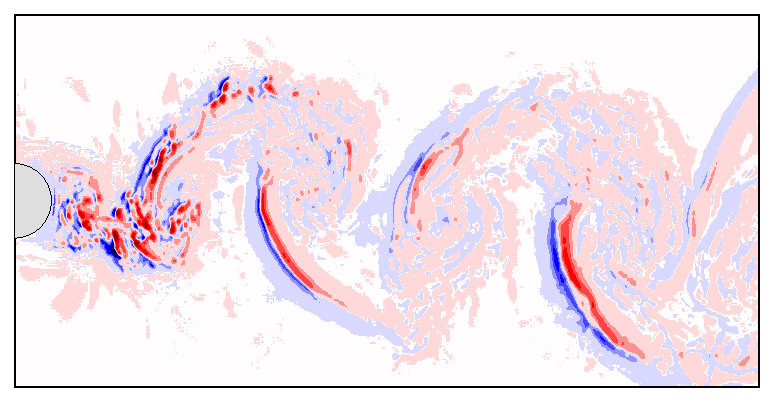
\includegraphics[width=\linewidth]{appendixD/predictions/SR_x_ML_raw_3693.0.pdf} \caption{$\mathcal{S}^{R,\,\mathrm{ML}}_x$ (raw)}
\end{subfigure}\vspace{0.5cm}
\begin{subfigure}[t]{\linewidth}
    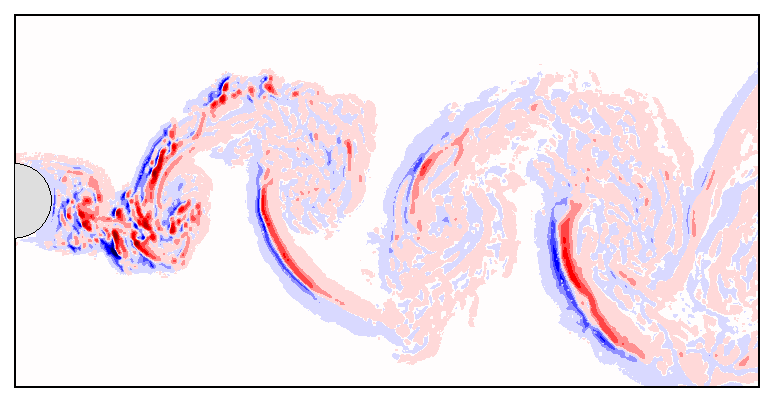
\includegraphics[width=\linewidth]{appendixD/predictions/SR_x_ML_pp_3693.0.pdf} \caption{$\mathcal{S}^{R,\,\mathrm{ML}}_x$ (post-processed)}
\end{subfigure}
\begin{subfigure}[t]{\linewidth}
    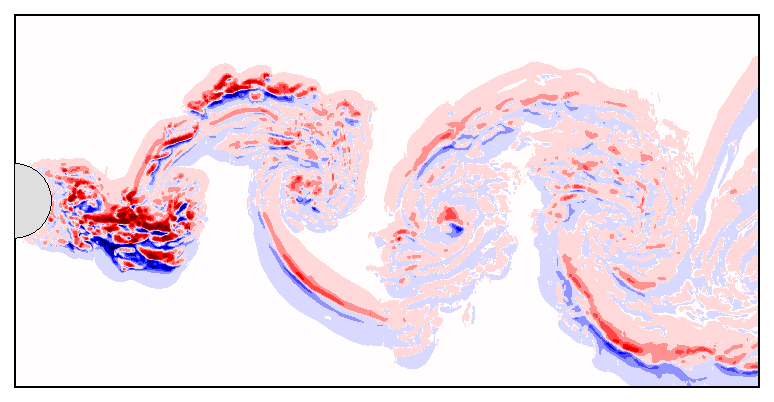
\includegraphics[width=\linewidth]{appendixD/predictions/SR_y_3693.0.pdf}\caption{$\mathcal{S}^R_y$}
\end{subfigure}\vspace{0.5cm}
\begin{subfigure}[t]{\linewidth}
    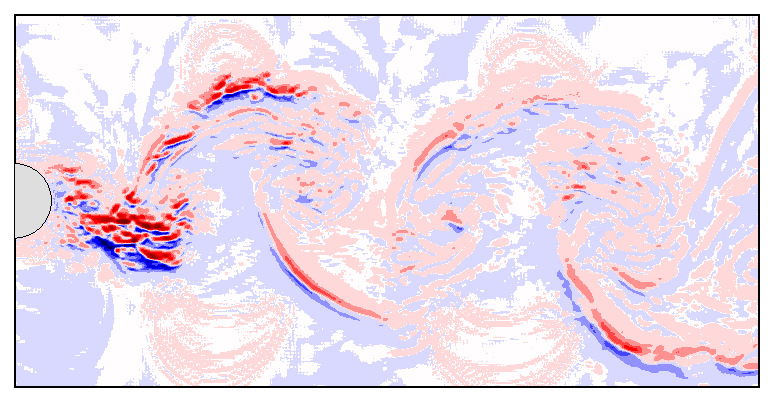
\includegraphics[width=\linewidth]{appendixD/predictions/SR_y_ML_raw_3693.0.pdf}\caption{$\mathcal{S}^{R,\,\mathrm{ML}}_y$ (raw)}
\end{subfigure}\vspace{0.5cm}
\begin{subfigure}[t]{\linewidth}
    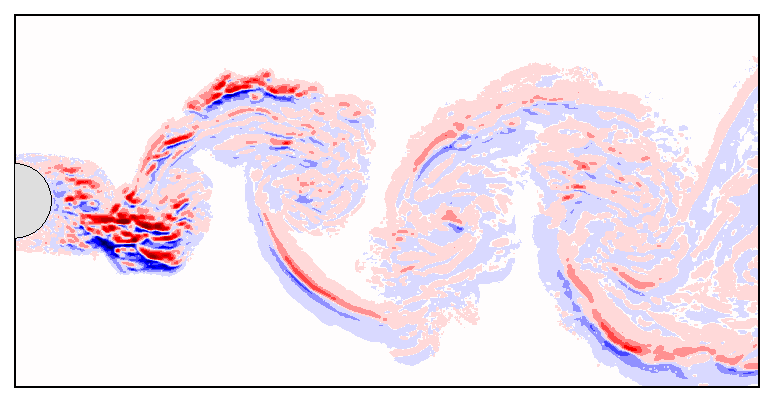
\includegraphics[width=\linewidth]{appendixD/predictions/SR_y_ML_pp_3693.0.pdf}\caption{$\mathcal{S}^{R,\,\mathrm{ML}}_y$ (post-processed)}
\end{subfigure}
\end{multicols}
\caption{Qualitative comparison between a snapshot of target fields (top), CNN raw predictions (middle), and CNN post-processed predictions (bottom).
The post-processing step removes high-frequency oscillations with a Gaussian filter and applies a wake detection filter constructed from the resolved vorticity field.}
\label{fig:predictions}
\end{figure*}
% ---------------------------------------------------------------- 
\end{document}